\section{Modello di sviluppo}
	Come modello di sviluppo si è deciso di provare ad utilizzare il \textbf{modello incrementale} (fig.1) in quanto risulta essere il più adatto allo sviluppo della componente software a noi richiesta in relazione alle nostre capacità. 
	
	\subsection{Modello Incrementale}
		Il modello incrementale o iterativo si basa sui seguenti passi:
		\begin{enumerate}
			\item pianificazione
			\item analisi dei requisiti
			\item progettazione
			\item implementazione
			\item validazione
			\item valutazione
		\end{enumerate}
		che possono essere eseguiti più volte, ma solo in maniera ciclica, da qui il nome "iterativo". Un approccio incrementale è consigliato quando la specifica dei requisiti risulta essere particolarmente difficoltosa e di difficile stesura, infatti questo modello favorisce lo sviluppo di prototipi che verranno utilizzati sia in fase di test che come anteprima per clienti

		\begin{figure}
			\centering
		    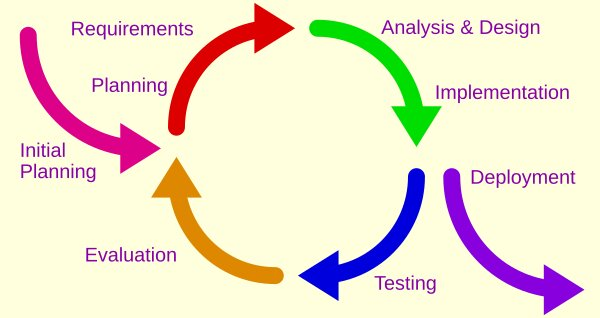
\includegraphics{Iterative_development_model.jpg}
			\caption{modello incrementale}\label{fig:1}
		\end{figure}